\chapter{SeqZip - Development and Applications} % Main chapter title
\label{Chapter2} 
\lhead{Chapter 2. \emph{SeqZip - Development and Applications}} 
%----------------------------------------------------------------------------------------
\section{SeqZip Overview}\label{sec: SeqZip Overview}
%----------------------------------------------------------------------------------------
% Write a lead-in to SeqZip development.
%-----------------------------------
\subsection{Subsection 1}\label{sec: SeqZip Overview}
%-----------------------------------


%% ############# FIGURE
\begin{figure}[htbp]
	\centering 
	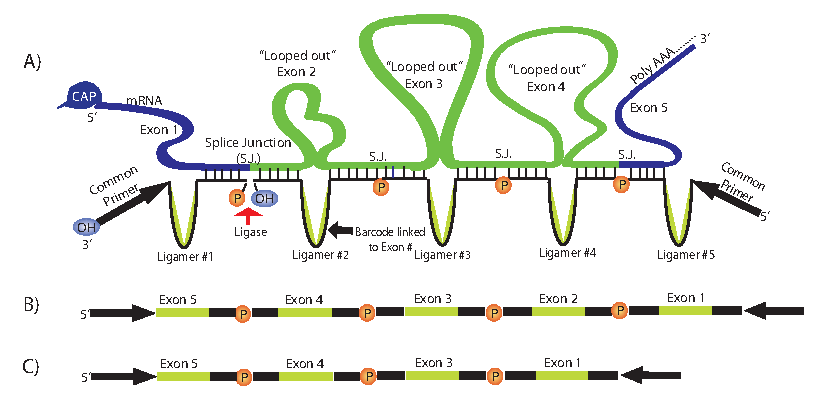
\includegraphics{Figures/Chapter2/OriginalSeqZipDiagram.pdf}
	\caption[Original SeqZip Diagram]
	{
		Original SeqZip Diagram\\
		This is the original concept diagram of the SeqZip methodology. (A) Specific DNA oligos target an mRNA and loop out the RNA sequence. Ligases is added to join the DNA oligos together; (B) \& (C) Two different possibilities of ligation products templated from the RNA in (A), where Exon 2 is an cassette exon.
	}
	\label{fig:Original SeqZip Diagram}
\end{figure}
%% ############# FIGURE

%----------------------------------------------------------------------------------------
\section{Multiplex Gene Study}
%----------------------------------------------------------------------------------------

One of the major goals of developing the SeqZip methodology was investigating potential coordination genome-wide. By genome-wide, what we really mean is to analyze many (or all) of the RNA transcripts in a tissue for evidence of coordinated splicing decisions. When development of the method reached the point that it could be applied in a multiplex study, I did not posses the bioinformatic skills necessary to 1) design ligamers in an automated and high-throughput fashion and 2) identify target transcripts, exons, and sequences to investigate for potential connectivity. Both of these points are discussed later, see <automated ligamer design | appendix> and <ideas on transcript identification for SeqZip coordination investigation | Discussion/Perspective>.

A hypothesis we wanted to use SeqZip to test was that coordination among distant regions of AS in the same transcript is a general phenomenon. It is important to note that we are not limiting our scope of coordination to that between two internal sites of AS (–e.g., cassette or mutually exclusive exon events). From microarrays studies, it has been estimated that approximately 30\% of all AS events involve alternative first and last exons (Bingham et al., 2008).  It is known that, through alternative use of first and last exons, cells can fine-tune a transcript’s untranslated region (UTR) and control many aspects of mRNA regulation including nuclear export, localization, expression, and stability (Hughes, 2006).  In support of the importance of alternative UTRs in tuning of gene expression, a landmark RNA-Seq study demonstrated a high occurrence of alternative first and last exon splicing, with alternative tandem 3’ UTR usage being the most highly tissue-dependent form of AS observed (Wang et al., 2008).  The current model of spatial proximity between 5’ and 3’ UTRs is suggestive of their possible interdependence. In our large-scale analysis, we included genes potentially displaying interdependence between first and last exons. Discovery of interdependence would lead to many questions into how specific combinations of UTRs can influence mRNA processing downstream of AS.


%% ############# FIGURE
\begin{figure}[htbp]
	\centering 
	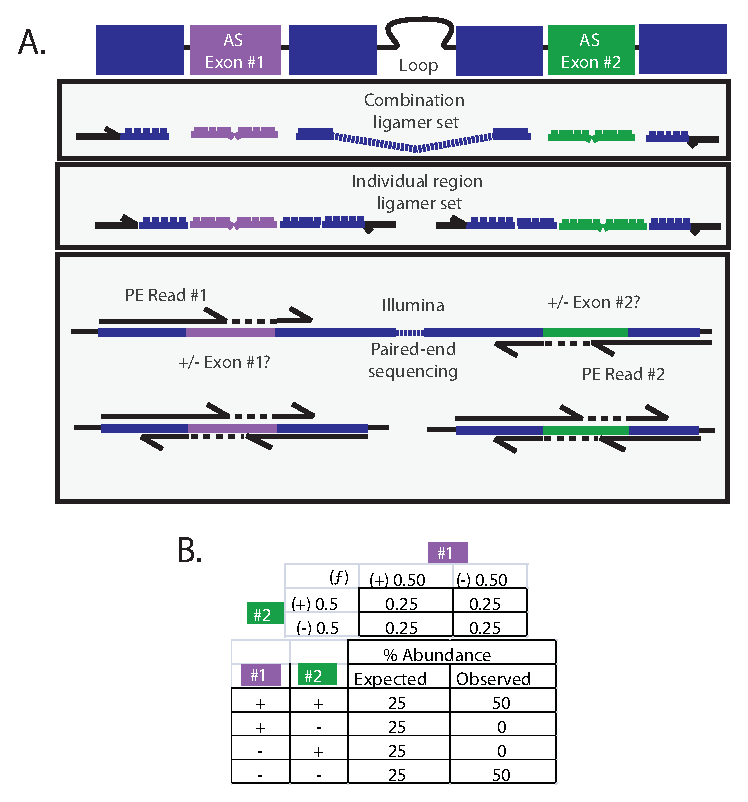
\includegraphics{Figures/Chapter2/10GeneSetSchematic.eps}
	\caption[10 Gene Set schematic]
	{
		10 Gene set schematic\\
		\hl{caption next}
	}
	\label{fig:Original SeqZip Diagram}
\end{figure}
%% ############# FIGURE

In an effort not to let my lack of bioinformatic ability hold back application of SeqZip to many transcripts at once, I designed a series of experiments that I termed a 'multiplex' application of SeqZip. It was based off of a very important paper from the Blencowe lab, where they used AS-sensitive microarrays to investigate transcripts in the Mouse CNS (Fagnani et al. 2007). This paper identified genes displaying tissue-specific splicing patterns, focusing on those with CNS-specific patterns. Once section of their paper focused on "Coordination between AS events belonging to the same genes," and seemed to be the exact type of experiment we were interested in applying the SeqZip method too. Five hundred of the 3,044 genes investigated by their microarrays contained 2–5 alternative exons. Fagnani et all contained an additional data file a list of all pair-wise combinations of alternative exons in the same gene (with that gene having significant expression in >20 different tissues), along with the standard and partial spearman correlations. Using this dataset, I filtered the exon pairs to those with a distance > 350 nt in the final pre-mRNA. I also visualized their transcript achetecture, and EST evidence using NCBIs AceView tool (Thierry-Mieg and Thierry-Mieg 2006). For example, the exons with strong correlation of expression in the Chl1 gene are in the beginning (second exon) and end (fourth from last exon, accession BC060216) with plenty of supporting evidence for these exons being expressed, and skipped.  After combing through the Fagnani data for a group of about 10 genes displaying these characteristics, I designed ligamers for the alternative, and flank constitutive exons. These oligos were then ordered from IDT in a 96-well plate format, pooled according to gene, and used to develop a multiplex approach to applying SeqZip, as well as investigate coordination between these exons, in these genes, using mouse total RNA from brains.

After synthesis, ligamers targeting a particular gene will be pooled at the predetermined appropriate concentration. Poly(A) samples from a treatment condition, cell-, or tissue-type of interest will be isolated.  These samples will be parsed out into individual wells of a 96-well plate, and different ligamer sets will be added to individual wells followed by analysis using SeqZip. Analysis of the resulting FLLPs can be carried out manually using semi-quantitative PCR, followed by denaturing PAGE or by one 454 sequencing run.  After analysis, the lengths of observed FLLPs will be related back to those predicted during ligamer construction.  Our primary data will represent the relative abundance of observed gene-specific isoforms for the cell- or tissue-type examined.

%-----------------------------------
\subsection{Subsection 1}
%-----------------------------------

\begin{table}[h]
\begin{tabular}{|l|r|r|r|r|}
\hline
\textbf{Gene name} & \textbf{nt of mRNA between exons} & \textbf{possible isoforms} & \textbf{Exon 1} & \textbf{Exon 2} \\ \hline
Chl1               & 4665                              & 18                         & 2               & 24              \\ \hline
Mdm1               & 1846                              & 4                          & EDA             & IIICS           \\ \hline
PTPRF-Y            & 1633                              & 4                          & 2               & 13              \\ \hline
Cacna1c            & 1403                              & 4                          & 15              & 21/22           \\ \hline
PTPRF-X            & 936                               & 4                          & 9/10            & 21              \\ \hline
FN1                & 813                               & 8                          & 13/14           & 21/22           \\ \hline
Apbb1              & 802                               & 260                        & 1/2b            & 2/3e            \\ \hline
Agrn               & 736                               & 8                          & 33/34c          & 33/34a          \\ \hline
Exoc7              & 513                               & 4                          & 7               & 13              \\ \hline
Prom1              & 512                               & 4                          & 7               & 9               \\ \hline
Lphn2              & 396                               & 32                         & 19              & 24/25a          \\ \hline
\end{tabular}
  \caption[Genes with big spans in between]{\hl{caption}}
  \label{BigSpanGenes}
\end{table}

%----------------------------------------------------------------------------------------
\section{Determining RNA integrity using SeqZip}\label{sec: SeqZip Intergrity}
%----------------------------------------------------------------------------------------

%-----------------------------------
\subsection{Demonstration of Concept}
%-----------------------------------

%% ############# FIGURE
\begin{figure}[htbp]
	\centering 
	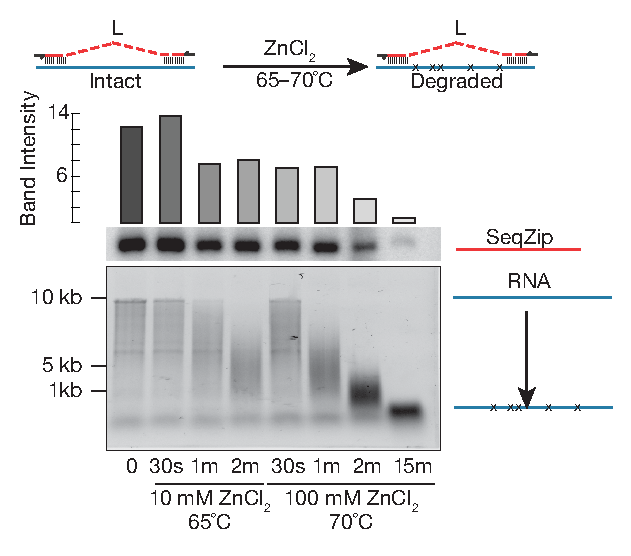
\includegraphics{Figures/Chapter2/DegreadedRNABySeqZip.eps}
	\caption[Ligation product tied to RNA integrity]
	{
		Ligation product tied to RNA integrity\\
		\hl{figure Caption}
	}
	\label{fig:Ligation product and RNA integrity}
\end{figure}
%% ############# FIGURE

\lipsum[1-3]

%% ############# FIGURE
\begin{figure}[htbp]
	\centering 
	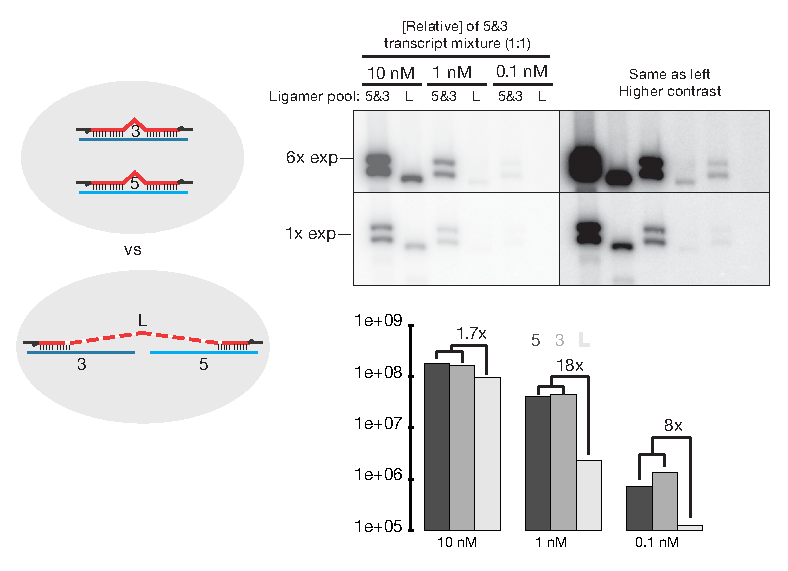
\includegraphics{Figures/Chapter2/TransRNAWithSeqZip.eps}
	\caption[Trans Transcript investigation]
	{
		Trans Transcript investigation\\
		\hl{figure Caption}
	}
	\label{fig:Ligation product and RNA integrity}
\end{figure}
%% ############# FIGURE

%-----------------------------------
\subsection{Investigating HIV viral genome integrity using SeqZip}
%-----------------------------------


%! Base the discussion off the introduction in the HIV paper (Serquiña et al. 2013)

MOV10L1 is implicated in HIV genome stability and intactness. We sought to measure the effects of a point mutant in the ATPase domain of MOV10L1 on the ‘intactness’ of the HIV genome. Viral particles contain two copies of the ssRNA HIV genome. Proteomics studies have measured MOV10L1 and Upf1 in viral particles, implicated these proteins, which are known helicases, in the maintained and infectivity of HIV.

%-----------------------------------
\subsection{Design of HIV ligamers}
%-----------------------------------

Research into the integrity of the HIV RNA genome using SeqZip began with designing a set of ligamers against two different clones. The first clone, targeting transcripts from the M19921 plasmid (so called 'M' clone), and transcripts from the K03455 clone contain nearly identical sequences with respect to the genome itself, and differ mostly in plasmid originating sequences. We targeted a difference in sequence for one site of ligation (Fig3-11A). Three different pools of ligamers were created initially: a Five(5) ligamer pool, with three ligamers design to test for the presence of sequence in the first 1,140 nt of the HIV genome, importantly the first site of ligation in the 5 region pool should contain a mismatch in the K clone sequence; a three(3) pool, testing the last 1,210 nt of the genome, and a Long (L) ligamer pool, also containing three ligamers, but the middle ligamer of which would span the 5 and 3 regions, looping out 8,633 nt of sequence in the middle of the HIV genome. In vitro transcripts were created using both the K and M clone plasmids. These transcripts were added to a background of total MEF RNA, and the SeqZIp assay was performed. Ligation products were successfully amplified from all ligamer pools when using the M clone transcript and all three ligamer pools. Also the abundance of these ligation products, as measured by endpoint PCR, seemed to be spike-concentration dependent. Notably, Ligation products were not obtained from the K clone using either the 5 or L ligamer pools, likely due to the mismatch between the transcript and the ligamers at the site of ligation. Also of note was the appearance of ligation products from purified endogenous virons of the M clone from all three ligamer pools, and the absence of products from virions purified from plasmids containing a defective protein, Gag, essential for viral packaging. 

%% ############# FIGURE
\begin{figure}[htbp]
	\centering 
	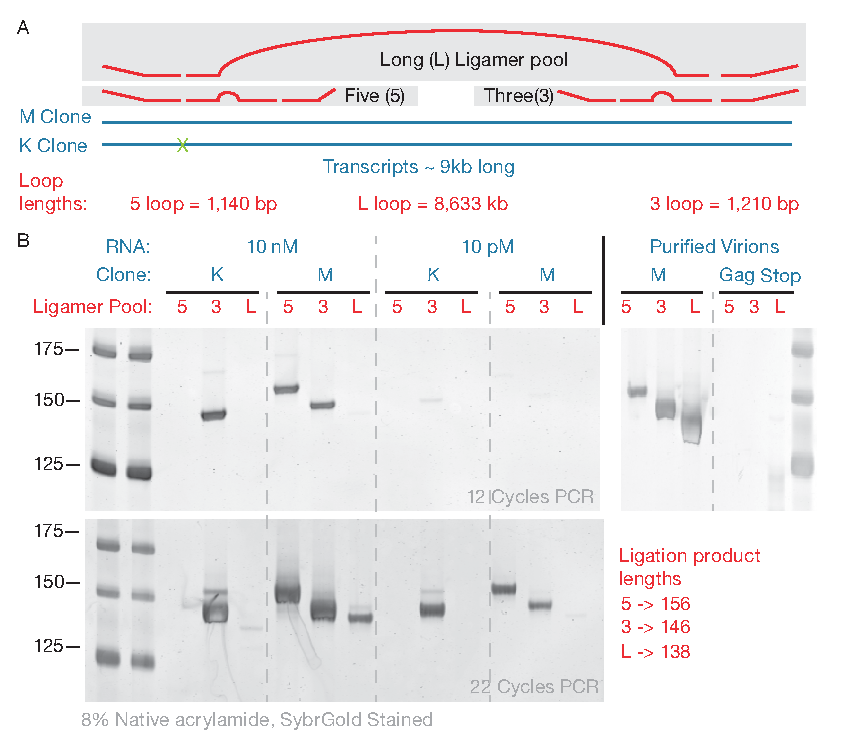
\includegraphics{Figures/Chapter2/HIVviaSeqZip.eps}
	\caption[SeqZip can examine HIV transcript integrity]
	{
		SeqZip can examine HIV transcript integrity\\
		\hl{figure Caption}
	}
	\label{fig:Hiv tx via SeqZip}
\end{figure}
%% ############# FIGURE

%----------------------------------------------------------------------------------------
\section{Continuity of piRNA precursor transcripts}\label{sec: piRNA Precursor SeqZip analysis}
%----------------------------------------------------------------------------------------

%% ############# FIGURE
\begin{figure}[htbp]
	\centering 
	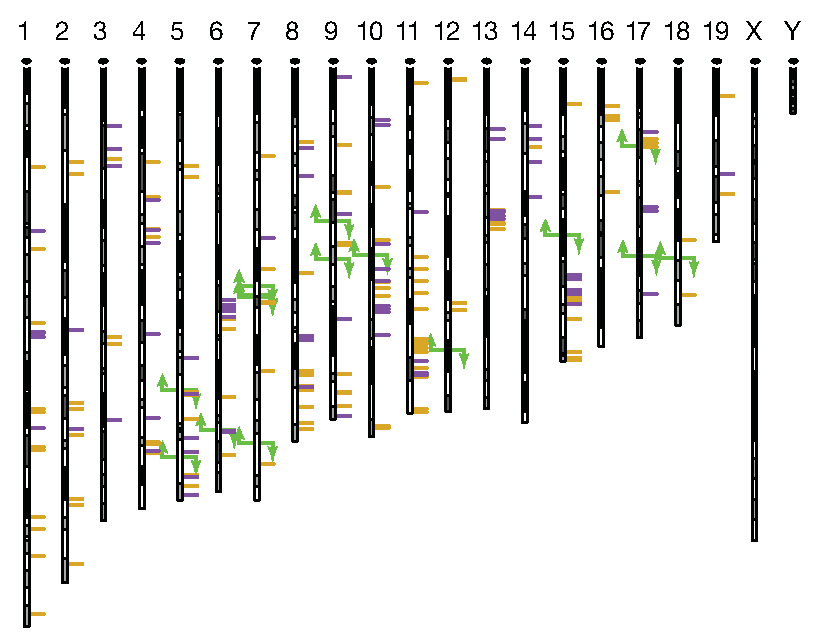
\includegraphics{Figures/Chapter2/PrecursorLocations.eps}
	\caption[piRNA precursor locations]
	{
		piRNA precursor locations\\
		\hl{figure Caption}
	}
	\label{fig:Hiv tx via SeqZip}
\end{figure}
%% ############# FIGURE


%Table 3 1, Just 9 clusters from 5 promoters generate >50% of 14.5 dpp (pachytene) piRNAs
\small
\begin{tabular}{llrrr}
\textbf{Cluster Name} & \textbf{\begin{tabular}[c]{@{}c@{}}Matched \\ Cluster\end{tabular}} & \textbf{\begin{tabular}[c]{@{}c@{}}Unique-mapping \\ piRNAs @ \\ wt.14dpp\end{tabular}} & \textbf{\begin{tabular}[c]{@{}c@{}}Fraction of \\ pachytene \\ piRNAs\end{tabular}} & \textbf{\begin{tabular}[c]{@{}c@{}}Cumulative\\  pachytene\\  piRNAs\end{tabular}} \\ \hline 
17-qA3.3-26735.1      & 17-qA3.3-27363                                                      & 3,021,022                                                                               & 17.2                                                                                & 17.2                                                                               \\        
17-qA3.3-27363.1      & 17-qA3.3-26735                                                      & 1,742,695                                                                               & 9.9                                                                                 & 27.2                                                                               \\        
9-qC-31469.1          & 9-qC-10667                                                          & 1,006,333                                                                               & 5.7                                                                                 & 32.9                                                                               \\        
9-qC-10667.1          & 9-qC-31469                                                          & 272,385                                                                                 & 1.6                                                                                 & 34.5                                                                               \\        
7-qD2-24830.1         & 7-qD2-11976                                                         & 652,564                                                                                 & 3.7                                                                                 & 38.2                                                                               \\        
7-qD2-11976.1         & 7-qD2-24830                                                         & 280,312                                                                                 & 1.6                                                                                 & 39.8                                                                               \\        
6-qF3-28913.1         & 6-qF3-8009                                                          & 564,930                                                                                 & 3.2                                                                                 & 43.0                                                                               \\        
6-qF3-8009.1          & 6-qF3-28913                                                         & 180,210                                                                                 & 1.0                                                                                 & 44.0                                                                               \\        
2-qE1-35981.1         & NA                                                                  & 1121042                                                                                 & 6.4                                                                                 & 50.4                                                                               \\ \hline 
\end{tabular}

%% ############# FIGURE
\begin{figure}[htbp]
	\centering 
	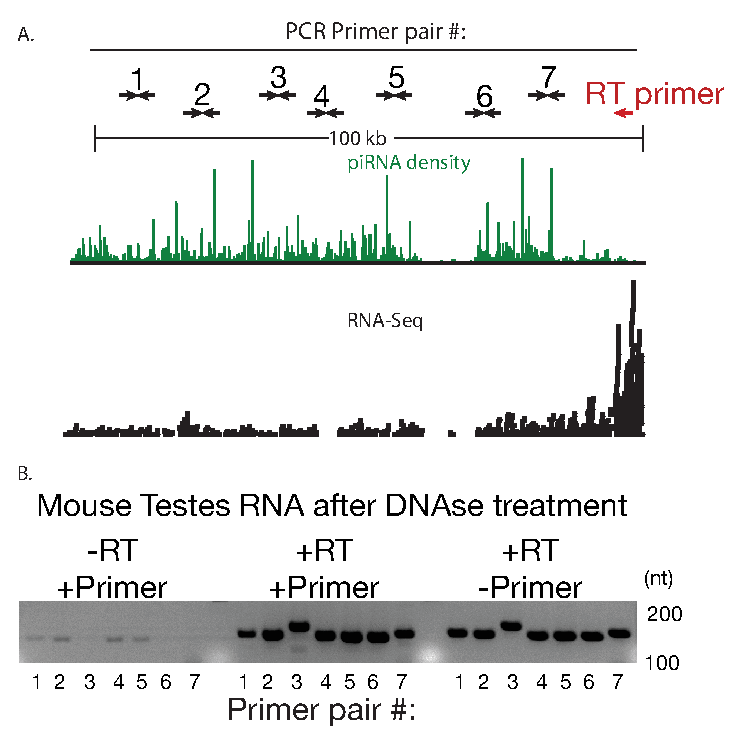
\includegraphics{Figures/Chapter2/RTDoesntWork.eps}
	\caption[pRT Doesn't Work for piRNA precursors]
	{
		RT Doesn't Work for piRNA precursors\\
		\hl{figure Caption}
	}
	\label{fig:Hiv tx via SeqZip}
\end{figure}
%% ############# FIGURE


%% ############# FIGURE
\begin{figure}[htbp]
	\centering 
	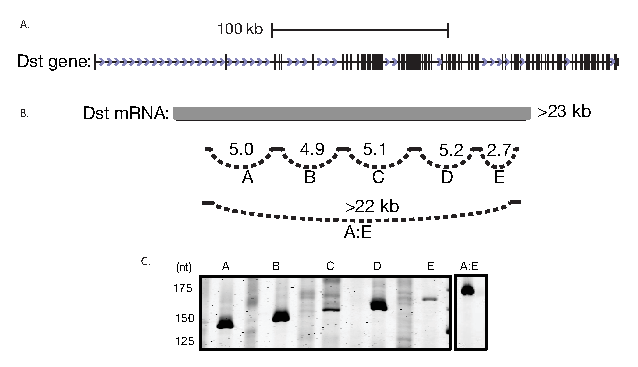
\includegraphics{Figures/Chapter2/dst1.eps}
	\caption[Dst1 by SeqZip]
	{
		Dst1 by SeqZip\\
		\hl{figure Caption}
	}
	\label{fig:Hiv tx via SeqZip}
\end{figure}
%% ############# FIGURE


%% ############# FIGURE
\begin{figure}[htbp]
	\centering 
	\includegraphics{Figures/Chapter2/testesSpecificRnaseqPrecursors.eps}
	\caption[Testes Specific RNA precursor expression]
	{
		Testes Specific RNA precursor expression\\
		\hl{figure Caption}
	}
	\label{fig:Hiv tx via SeqZip}
\end{figure}
%% ############# FIGURE


%% ############# FIGURE
\begin{figure}[htbp]
	\centering 
	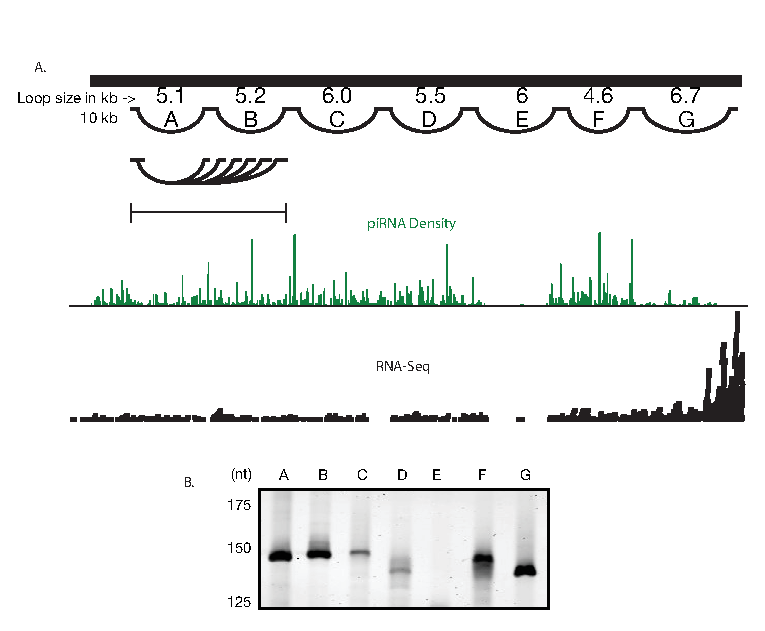
\includegraphics{Figures/Chapter2/piRNAPrecurserAnalyisBySeqZip.eps}
	\caption[piRNA precursor analysis via SeqZip]
	{
		piRNA precursor analysis via SeqZip\\
		\hl{figure Caption}
	}
	\label{fig:Hiv tx via SeqZip}
\end{figure}
%% ############# FIGURE


